\documentclass[12pt, a4paper, oneside]{ctexart}
\usepackage{amsmath, amsthm, amssymb, bm, color, graphicx, geometry, mathrsfs,extarrows, braket, booktabs, array}
\usepackage[colorlinks,linkcolor=red,anchorcolor=blue,citecolor=blue,urlcolor=blue,menucolor=black]{hyperref}
\setmainfont{Times New Roman}  % 设置英文字体
\setsansfont{Calibri}
\setmonofont{Consolas}

\linespread{1.4}
%\geometry{left=2.54cm,right=2.54cm,top=3.18cm,bottom=3.18cm}
\geometry{left=1.84cm,right=1.84cm,top=2.18cm,bottom=2.18cm}
\newcounter{problem}  % 问题序号计数器
\newenvironment{problem}{\stepcounter{problem}\par\noindent\textbf{题目\arabic{problem}. }}{\smallskip\par}
\newenvironment{solution}{\par\noindent\textbf{解答. }}{\smallskip\par}
\newenvironment{note}{\par\noindent\textbf{注记. }}{\smallskip\par}

%%%% 图片相对路径 %%%%
\graphicspath{{figure/}} % 当前目录下的figure文件夹, {../figure/}则是父目录的figure文件夹

\everymath{\displaystyle} % 默认全部行间公式
\DeclareMathOperator*\uplim{\overline{lim}} % 定义上极限 \uplim_{}
\DeclareMathOperator*\lowlim{\underline{lim}} % 定义下极限 \lowlim_{}
\let\leq=\leqslant % 将全部leq变为leqslant
\let\geq=\geqslant % geq同理
\DeclareRobustCommand{\rchi}{{\mathpalette\irchi\relax}}
\newcommand{\irchi}[2]{\raisebox{\depth}{$#1\chi$}} % 使用\rchi将\chi居中

%%%% 一些宏定义 %%%%
\def\bd{\boldsymbol}        % 加粗(向量) boldsymbol
\def\disp{\displaystyle}    % 使用行间公式 displaystyle(默认)
\def\tsty{\textstyle}       % 使用行内公式 textstyle
\def\sign{\text{sign}}      % sign function
\def\wtd{\widetilde}        % 宽波浪线 widetilde
\def\R{\mathbb{R}}          % Real number
\def\N{\mathbb{N}}          % Natural number
\def\Z{\mathbb{Z}}          % Integer number
\def\Q{\mathbb{Q}}          % Rational number
\def\C{\mathbb{C}}          % Complex number
\def\d{\mathrm{d}}          % differential operator
\def\e{\mathrm{e}}          % Euler's number
\def\i{\mathrm{i}}          % imaginary number
\def\E{\mathrm{E}}          % Exception
\def\P{\mathrm{P}}          % 概率
\def\var{\mathrm{Var}}      % 方差
\def\re{\mathrm{Re}}        % Real part
\def\im{\mathrm{Im}}        % Imaginary part
\def\res{\mathrm{Res}}      % Residue
\def\L{\mathcal{L}}         % Loss function
\def\wdh{\widehat}          % 宽帽子 widehat
\def\ol{\overline}          % 上横线 overline
\def\ul{\underline}         % 下横线 underline
\def\add{\vspace{1ex}}      % 增加行间距
\def\del{\vspace{-3.5ex}}   % 减少行间距

%%%% 定理类环境的定义 %%%%
\newtheorem{theorem}{定理}

%%%% 基本信息 %%%%
\newcommand{\RQ}{\today} % 日期
\newcommand{\km}{数理统计} % 科目
\newcommand{\bj}{强基数学002} % 班级
\newcommand{\xm}{吴天阳} % 姓名
\newcommand{\xh}{2204210460} % 学号

\begin{document}

%\pagestyle{empty}
\pagestyle{plain}
\vspace*{-15ex}
\centerline{\begin{tabular}{*5{c}}
    \parbox[t]{0.25\linewidth}{\begin{center}\textbf{日期}\\ \large \textcolor{blue}{\RQ}\end{center}} 
    & \parbox[t]{0.2\linewidth}{\begin{center}\textbf{科目}\\ \large \textcolor{blue}{\km}\end{center}}
    & \parbox[t]{0.2\linewidth}{\begin{center}\textbf{班级}\\ \large \textcolor{blue}{\bj}\end{center}}
    & \parbox[t]{0.1\linewidth}{\begin{center}\textbf{姓名}\\ \large \textcolor{blue}{\xm}\end{center}}
    & \parbox[t]{0.15\linewidth}{\begin{center}\textbf{学号}\\ \large \textcolor{blue}{\xh}\end{center}} \\ \hline
\end{tabular}}
\vspace*{4ex}

% 正文部分
\begin{problem}
    如果$X_1,\cdots, X_n$是来自$N(\mu,\sigma^2)$的随机样本,求样本标准差$S=\sqrt{\frac{\sum_{i=1}^n(X_i-\bar{X})^2}{n-1}}$的期望与方差.
\end{problem}
\begin{solution}
    令$Y = \frac{(n-1)S^2}{\sigma^2}$则$Y\sim \rchi(n-1)$,由于$S = \frac{\sigma}{\sqrt{n-1}}\sqrt{Y}$,于是
    \begin{align*}
        \E(\sqrt{Y}) =&\ \frac{\sigma}{\sqrt{n-1}}\int_0^\infty\sqrt{x}\cdot\frac{(\frac{1}{2})^{\frac{n-1}{2}}}{\Gamma(\frac{n-1}{2})}x^{\frac{n-1}{2}-1}e^{-\frac{x}{2}}\,\d x = \frac{(\frac{1}{2})^{\frac{n-1}{2}}}{\Gamma(\frac{n-1}{2})}\int_0^\infty x^{\frac{n}{2}-1}e^{-\frac{x}{2}}\,\d x\\
        =&\ \frac{(\frac{1}{2})^{\frac{n-1}{2}}}{\Gamma(\frac{n-1}{2})}\cdot\frac{\Gamma(\frac{n}{2})}{(\frac{1}{2})^{\frac{n}{2}}} = \frac{\sqrt{2}\Gamma(\frac{n}{2})}{\Gamma(\frac{n-1}{2})}
    \end{align*}
    所以$\E(S) = \frac{\sigma}{\sqrt{n-1}}\E(\sqrt{Y}) = \frac{\sqrt{2}\sigma\Gamma(\frac{n}{2})}{\sqrt{n-1}\Gamma(\frac{n-1}{2})}$.

    由样本方差性质可知$\E(S^2) = \sigma^2$,于是$\var(S) = \E(S^2) - \E(S)^2 = \sigma^2 - \frac{\sqrt{2}\sigma\Gamma(\frac{n}{2})}{\sqrt{n-1}\Gamma(\frac{n-1}{2})} = \sigma^2\left(1 - \frac{2}{n-1}\cdot\frac{\Gamma^2(\frac{n}{2})}{\Gamma^2(\frac{n-1}{2})}\right)$.
\end{solution}
\begin{problem}
    如果$X_1,\cdots, X_n$是来自均匀分布总体$U(0,1)$的随机样本,求$Y = \left(\prod_{i=1}^nX_i\right)^{-\frac{1}{n}}$的分布.
\end{problem}
\begin{solution}
    由于$\log Y = \frac{1}{n}\sum_{i=1}^n-\log X_i$,令$Z = -\log X$,则
    \begin{equation*}
        f_Z(z) = f_X(\e^{-z})\cdot |-\e^{-z}| = \e^{-z},
    \end{equation*}
    则$-\log X_i = Z\sim \Gamma(1, 1)$. 令$U = \sum_{i=1}^n-\log X_i$,则由Gamma函数的可加性可知,$U\sim \Gamma(n, 1)$,于是
    \begin{equation*}
        f_{\frac{U}{n}}(x) = f_U(nx)\cdot n = \frac{n}{\Gamma(n)}(nx)^{n-1}\e^{-x} = \frac{n^n}{\Gamma(n)}x^{n-1}\e^{-x},
    \end{equation*}
    所以
    \begin{equation*}
        f_Y(y) = f_{\log Y}(e^y) = f_{\frac{U}{n}}(\e^y)\cdot \e^y = \frac{n^n}{\Gamma(n)}\e^{ny}\e^{-\e^{y}}.
    \end{equation*}
\end{solution}
\begin{problem}
    设$X_1,X_2$是来自$N(0,1)$的随机样本.
    
    (1) 求$(X_2-X_1)/\sqrt{2}$的分布.

    (2) 求$X_1^2+X_2^2$的分布.

    (3) 求$(X_1+X_2)^2/(X_2-X_1)^2$的分布.

    (4) 求$(X_2+X_1)/\sqrt{(X_1-X_2)^2}$的分布.

    (5) 求$X_1^2/X_2^2$的分布.
\end{problem}
\begin{solution}
    (1) 由正态分布的线性性可知$X_2-X_1\sim N(0, 2)$,于是$(X_2-X_1) / \sqrt{2}\sim N(0,1)$.

    (2) 由卡方分布性质可知$X_1^2+X_2^2\sim \rchi(2)$.

    (3) 由卡方分布性质可知$(X_1+X_2)^2/2\sim\rchi(1),\ (X_2-X_1)^2/2\sim\rchi(1)$,再由$F$分布的性质可知$(X_1+X_2)^2/(X_2-X_1)^2\sim F(1, 1)$.

    (4) 由正态分布性质可知$(X_2+X_1)/\sqrt{2}\sim N(0,1)$,$(X_1-X_2)^2/2\sim \rchi(1)$,再由$t$分布的性质可知$(X_2+X_1)/\sqrt{(X_1-X_2)^2}\sim t(1)$.

    (5) 由卡方分布性质可知$X_1^2,X_2^2\sim \chi(1)$,再由$F$分布可知$X_1^2/X_2^2\sim F(1,1)$.
\end{solution}
\begin{problem}
    设$X_1,\cdots,X_n$是来自总体$X$的随机样本,$\E(X) = \mu$,且$\var(X) = 0.25$,假设至少以$95\%$的概率保证$|\bar{X}-\mu| < 0.001$,问样本量$n$至少应取多大?
\end{problem}
\begin{solution}
    由Chebyshev不等式可知
    \begin{equation*}
        \P(|\bar{X}-\mu|>\varepsilon) = \P(|\bar{X}-\mu|^2 > \varepsilon^2)\leq\frac{|\bar{X}-\mu|^2}{\varepsilon^2}=\frac{\sigma^2}{n\varepsilon^2}
    \end{equation*}
    取$\varepsilon = 0.01$,则$\frac{0.25}{n(0.01)^2}\leq 0.05\Rightarrow n\geq 500$,则$n$至少为$500$.
\end{solution}
\begin{problem}
    如果$X$服从自由度为$m$和$n$的$F$分布.\add

    (1) 求$W = \frac{mX/n}{1+mX/n}$的分布.

    (2) 根据$(1)$的计算结果,计算$X$的期望与方差.
\end{problem}
\begin{solution}
    (1) 设两个独立的随机变量$U\sim\rchi^2(m), V\sim\rchi^2(n)$,有$F$分布的性质可知,$X = \frac{U/m}{V/n}\sim F(m, n)$,于是$W = \frac{U}{U+V}$. 做变量代换如下
    \begin{equation*}
        \begin{cases}
            x = \frac{u}{u+v},\\
            u = v.
        \end{cases}\Rightarrow\begin{cases}
            u = \frac{xy}{1-x},\\
            v = y.
        \end{cases}\Rightarrow \text{det}(J) = \left|\begin{matrix}
            \frac{y}{(1-x)^2}&\frac{x}{1-x}\\0&1
        \end{matrix}\right|=\frac{2-x}{(1-x)^2}y.
    \end{equation*}
    则
    \begin{equation*}
        p(x,y) = p_{U,V}\left(\frac{xy}{1-x},y\right)=\frac{(\frac{1}{2})^{\frac{m+n}{2}}}{\Gamma(\frac{m}{2})\Gamma(\frac{n}{2})}\frac{x^{\frac{m}{2}-1}}{(1-x)^{\frac{m}{2}+1}}y^{\frac{m+n}{2}-1}\e^{-\frac{y}{2(1-x)}}
    \end{equation*}
    于是
    \begin{equation*}
        p_W(x) = \int_0^\infty p(x,y)\,\d y\xlongequal{\text{凑}\Gamma\text{函数}}\frac{(\frac{1}{2})^{\frac{m+n}{2}}}{\Gamma(\frac{m}{2})\Gamma(\frac{n}{2})}\frac{x^{\frac{m}{2}-1}}{(1-x)^{\frac{m}{2}+1}}\frac{\Gamma(\frac{m+n}{2})}{\left(\frac{1}{2(1-x)}\right)^{\frac{m+n}{2}}} = \frac{\Gamma(\frac{m+n}{2})}{\Gamma(\frac{m}{2})\Gamma(\frac{n}{2})}x^{\frac{m}{2}-1}(1-x)^{\frac{n}{2}-1}
    \end{equation*}
    所以$W\sim Beta\left(\frac{m}{2},\frac{n}{2}\right)$.

    (2) 由于$W = \frac{mX}{n+mX}\Rightarrow X = \frac{n}{m}\cdot\frac{W}{1-W}$,则
    \begin{align*}
        \E(X) = \frac{n}{m}\E\left(\frac{W}{1-W}\right) =&\ \frac{n}{m}\,\frac{\Gamma(\frac{m+n}{2})}{\Gamma(\frac{m}{2})\Gamma(\frac{n}{2}))}\int_0^1w^{\frac{m}{2}}(1-w)^{\frac{n}{2}-2}\,\d w\\
        \xlongequal{\text{凑}Beta\text{分布}}&\ \frac{n}{m}\,\frac{\Gamma(\frac{m+n}{2})}{\Gamma(\frac{m}{2})\Gamma(\frac{n}{2}))}\,\frac{\Gamma(\frac{m}{2}+1)\Gamma(\frac{n}{2}-1))}{\Gamma(\frac{m+n}{2})} = \frac{n}{m}\,\frac{m/2}{n/2-1}=\frac{n}{n-2}.
    \end{align*}
    \begin{align*}
        \E(X^2) = \frac{n^2}{m^2}\E\left(\frac{W^2}{(1-W)^2}\right) =&\ \frac{n^2}{m^2}\frac{\Gamma(\frac{m+n}{2})}{\Gamma(\frac{m}{2})\Gamma(\frac{n}{2})}\int_0^1w^{\frac{m}{2}+1}(1-w)^{\frac{n}{2}-3}\,\d w\\
        \xlongequal{\text{凑}Beta\text{分布}}&\ \frac{n^2}{m^2}\,\frac{\Gamma(\frac{m+n}{2})}{\Gamma(\frac{m}{2})\Gamma(\frac{n}{2})}\,\frac{\Gamma(\frac{m}{2}+2)\Gamma(\frac{n}{2}-2)}{\Gamma(\frac{m+n}{2})} = \frac{n^2(m+2)}{m(n-4)(n-2)}
    \end{align*}
    \begin{align*}
        \var(X) = \E(X^2)-\E(X)^2 = \frac{n^2(m+2)}{m(n-4)(n-2)} - \frac{n^2}{(n-2)^2} = \frac{2n^2(n+m-2)}{m(n-4)(n-2)^2}.
    \end{align*}
\end{solution}

% 下面给一些功能的写法
\iffalse
% 图片模板
\centerline{
    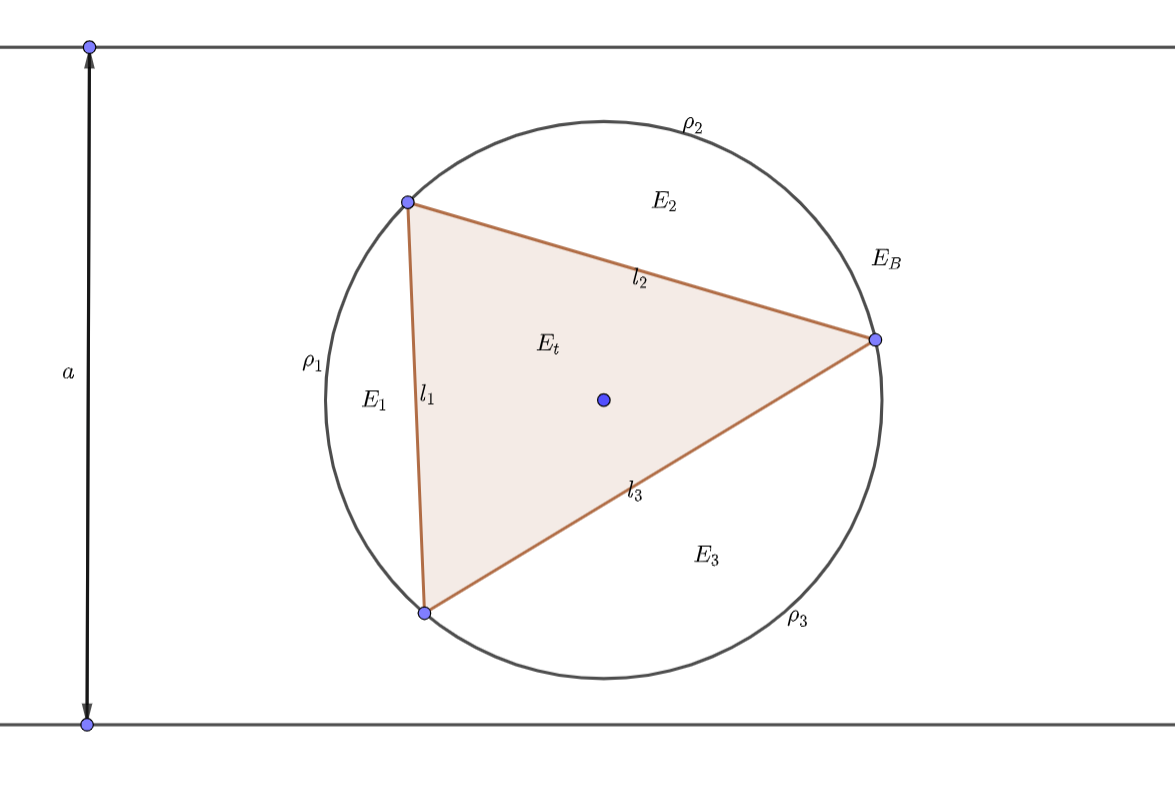
\includegraphics[width=0.8\textwidth]{figure.png}
}
% 表格模板
\renewcommand\arraystretch{0.8} % 设置表格高度为原来的0.8倍
\begin{table}[!htbp] % table标准
    \centering % 表格居中
    \begin{tabular}{p{1cm}<{\centering}p{1cm}<{\centering}p{3cm}<{\centering}p{5cm}<{\centering}} % 设置表格宽度
    %\begin{tabular}{cccc}
        \toprule
        $x_i$ & $f[x_1]$ & $f[x_i,x_{i+1}]$ & $f[x_i,x_{i+1},x_{i+2}]$ \\
        \midrule
        $x_0$ & $f(x_0)$ &                  &                          \\
        $x_0$ & $f(x_0)$ & $f'(x_0)$        &                          \\
        $x_0$ & $f(x_1)$ & $\frac{f(x_1)-f(x_0)}{x_1-x_0}$ & $\frac{f(x_1)-f(x_0)}{(x_1-x_0)^2}-\frac{f'(x_0)}{x_1-x_0}$\\
        \bottomrule
    \end{tabular}
\end{table}

\def\Log{\text{Log}} % 一个简单的宏定义
$\Log$ % 调用方法
\fi

\end{document}